%%%%%%%%%%%%%%%%%%%%%%%%%%%%%%%%%%%%%%%%%
% Beamer Presentation - LaTeX Template
% Version 2.0 (March 8, 2022)
% Original Template: https://www.LaTeXTemplates.com
% Author: Vel (vel@latextemplates.com)
% License: CC BY-NC-SA 4.0

% Este modelo de apresentação foi 
% criado a partir do modelo de Giovanni Spadaro.
% Disponível em: https://github.com/Giovo17/presentation-template-unict-lm-data
%
% Adaptado por Lucas Amaral Taylor para criar uma versão especial 
% para os alunos de Matemática e Estatística da USP (IME-USP).
% Disponível em: https://github.com/lucasamtaylor01/IME-template
%%%%%%%%%%%%%%%%%%%%%%%%%%%%%%%%%%%%%%%%%

%----------------------------------------------------------------------------------------
% CLASSE DO DOCUMENTO E CONFIGURAÇÕES BÁSICAS
%----------------------------------------------------------------------------------------
\documentclass[
    11pt,               % Tamanho padrão da fonte
    % t,                % Alinhar verticalmente ao topo
    %aspectratio=169,   % Definir proporção 16:9
]{beamer}
\graphicspath{{img/}}         % Define o diretório das imagens

%----------------------------------------------------------------------------------------
% PACOTES NECESSÁRIOS
%----------------------------------------------------------------------------------------
\usepackage{
    booktabs,     % Melhora a aparência das linhas em tabelas
     palatino,     % Define Palatino como fonte principal
    subcaption    % Suporte para subfiguras
}
\usepackage[dvipsnames]{xcolor} 
\usepackage{tcolorbox}
\usepackage[default]{opensans}  % Define Open Sans como fonte secundária
%----------------------------------------------------------------------------------------
%	PACOTES E CONFIGURAÇÕES PARA CÓDIGO
%----------------------------------------------------------------------------------------
% Pacotes necessários para formatação de código
\usepackage[utf8]{inputenc}
\usepackage{listings}
\usepackage{xcolor}

% Cores para syntax highlighting (VSCode Light Theme)
\definecolor{vscBackground}{RGB}{255,255,255}    % Fundo branco
\definecolor{vscKeyword}{RGB}{175,0,219}         % Roxo para palavras-chave
\definecolor{vscString}{RGB}{163,21,21}          % Vermelho para strings
\definecolor{vscComment}{RGB}{0,128,0}           % Verde para comentários
\definecolor{vscFunction}{RGB}{121,94,38}        % Marrom para funções
\definecolor{vscNumber}{RGB}{9,134,88}           % Verde escuro para números
\definecolor{vscOperator}{RGB}{175,0,219}        % Roxo para operadores
\definecolor{vscText}{RGB}{0,0,0}                % Texto preto
\definecolor{vscLineNr}{RGB}{128,128,128}
\definecolor{lusoCustom}{RGB}{247,247,247}% Cinza para números de linha
\definecolor{luso2}{RGB}{207,207,207}% Cinza para números de linha

% Configuração geral do listings para UTF-8
\lstset{
    inputencoding=utf8,
    extendedchars=true,
    literate=%
        {á}{{\'a}}1 {é}{{\'e}}1 {í}{{\'i}}1 {ó}{{\'o}}1 {ú}{{\'u}}1
        {Á}{{\'A}}1 {É}{{\'E}}1 {Í}{{\'I}}1 {Ó}{{\'O}}1 {Ú}{{\'U}}1
        {à}{{\`a}}1 {è}{{\`e}}1 {ì}{{\`i}}1 {ò}{{\`o}}1 {ù}{{\`u}}1
        {À}{{\`A}}1 {È}{{\'E}}1 {Ì}{{\`I}}1 {Ò}{{\`O}}1 {Ù}{{\`U}}1
        {ã}{{\~a}}1 {ẽ}{{\~e}}1 {ĩ}{{\~i}}1 {õ}{{\~o}}1 {ũ}{{\~u}}1
        {Ã}{{\~A}}1 {Ẽ}{{\~E}}1 {Ĩ}{{\~I}}1 {Õ}{{\~O}}1 {Ũ}{{\~U}}1
        {â}{{\^a}}1 {ê}{{\^e}}1 {î}{{\^i}}1 {ô}{{\^o}}1 {û}{{\^u}}1
        {Â}{{\^A}}1 {Ê}{{\^E}}1 {Î}{{\^I}}1 {Ô}{{\^O}}1 {Û}{{\^U}}1
        {ç}{{\c c}}1 {Ç}{{\c C}}1
        {º}{{\textordmasculine}}1
        {ª}{{\textordfeminine}}1
}

% Configurações base comum para todas as linguagens
\lstdefinestyle{baseStyle}{
    backgroundcolor=\color{vscBackground},
    basicstyle=\ttfamily\tiny\color{vscText},
    breakatwhitespace=false,
    breaklines=true,
    captionpos=b,
    keepspaces=true,
    numbers=left,
    numbersep=5pt,
    showspaces=false,
    showstringspaces=false,
    showtabs=false,
    tabsize=4,
    frame=single,
    framerule=1pt,
    rulecolor=\color{gray!20},
    numberstyle=\tiny\color{vscLineNr},
    keywordstyle=\color{vscKeyword},
    commentstyle=\color{vscComment}\itshape,
    stringstyle=\color{vscString},
    emphstyle=\color{vscFunction},
    columns=flexible,
    basewidth={0.5em,0.45em},
    inputencoding=utf8,
    extendedchars=true
}

\newtcolorbox{roundedcodebox}{
    colback={lusoCustom}, % Background color
    colframe=luso2, % Border color
    rounded corners, % Enables rounded edges
    boxrule=0.5pt, % Border thickness
}

%----------------------------------------------------------------------------------------
% Python
%----------------------------------------------------------------------------------------
\lstdefinestyle{pythonStyle}{
    style=baseStyle,
    language=Python,
    morekeywords={self,None,True,False,import,from,as,def,class,return,yield,
                  for,while,if,else,elif,try,except,finally,with,lambda,
                  async,await,break,continue,global,nonlocal,pass,raise},
    morekeywords=[2]{print,len,range,type,int,str,float,list,dict,set,
                     tuple,max,min,sum,sorted,enumerate,zip,map,filter,
                     any,all,abs,round,pow,divmod},
    keywordstyle=[2]\color{vscFunction},
    sensitive=true
}

\lstnewenvironment{python}[1][]{\lstset{style=pythonStyle, #1}}{}
\newcommand{\pyinline}[1]{\lstinline[style=pythonStyle]!#1!}
\newcommand{\inputpython}[2][]{\lstinputlisting[style=pythonStyle,#1]{#2}}

%----------------------------------------------------------------------------------------
% C Language
%----------------------------------------------------------------------------------------
\lstdefinestyle{cStyle}{
    style=baseStyle,
    language=C,
    morekeywords={include,define,void,int,char,float,double,long,unsigned,
                  struct,union,enum,typedef,const,static,extern,register,
                  auto,volatile,sizeof,return,if,else,for,while,do,switch,
                  case,break,continue,default,goto},
    morekeywords=[2]{printf,scanf,malloc,free,calloc,realloc,fopen,fclose,
                     fprintf,fscanf,strcpy,strlen,strcat},
    keywordstyle=[2]\color{vscFunction},
    sensitive=true
}

\lstnewenvironment{clang}[1][]{\lstset{style=cStyle, #1}}{}
\newcommand{\clinline}[1]{\lstinline[style=cStyle]!#1!}
\newcommand{\inputclang}[2][]{\lstinputlisting[style=cStyle,#1]{#2}}

%----------------------------------------------------------------------------------------
% C++
%----------------------------------------------------------------------------------------
\lstdefinestyle{cppStyle}{
    style=baseStyle,
    language=C++,
    morekeywords={class,private,protected,public,template,typename,namespace,
                  using,new,delete,this,friend,virtual,override,final,explicit,
                  mutable,constexpr,nullptr,noexcept,static_cast,dynamic_cast,
                  const_cast},
    morekeywords=[2]{cout,cin,endl,vector,string,map,set,queue,stack,pair,
                     begin,end,push_back,pop_back,emplace_back,size,empty},
    keywordstyle=[2]\color{vscFunction},
    sensitive=true
}

\lstnewenvironment{cpp}[1][]{\lstset{style=cppStyle, #1}}{}
\newcommand{\cppinline}[1]{\lstinline[style=cppStyle]!#1!}
\newcommand{\inputcpp}[2][]{\lstinputlisting[style=cppStyle,#1]{#2}}

%----------------------------------------------------------------------------------------
% R Language
%----------------------------------------------------------------------------------------
\lstdefinestyle{rStyle}{
    style=baseStyle,
    language=R,
    morekeywords={if,else,repeat,while,function,for,in,next,break,TRUE,FALSE,
                  NULL,Inf,NaN,NA,NA_integer_,NA_real_,NA_complex_,NA_character_},
    morekeywords=[2]{library,require,attach,detach,source,setwd,options,
                     data.frame,read.csv,write.csv,list,matrix,array},
    keywordstyle=[2]\color{vscFunction},
    sensitive=true
}

\lstnewenvironment{rlang}[1][]{\lstset{style=rStyle, #1}}{}
\newcommand{\rlinline}[1]{\lstinline[style=rStyle]!#1!}
\newcommand{\inputrlang}[2][]{\lstinputlisting[style=rStyle,#1]{#2}}

%----------------------------------------------------------------------------------------
% Java
%----------------------------------------------------------------------------------------
\lstdefinestyle{javaStyle}{
    style=baseStyle,
    language=Java,
    morekeywords={abstract,assert,boolean,break,byte,case,catch,char,class,
                  const,continue,default,do,double,else,enum,extends,final,
                  finally,float,for,if,implements,import,instanceof,int,
                  interface,long,native,new,package,private,protected,public,
                  return,short,static,strictfp,super,switch,synchronized,this,
                  throw,throws,transient,try,void,volatile,while},
    morekeywords=[2]{String,System,out,println,printStackTrace,ArrayList,
                     HashMap,Arrays,List,Map,Set,Exception,RuntimeException},
    keywordstyle=[2]\color{vscFunction},
    sensitive=true
}

\lstnewenvironment{java}[1][]{\lstset{style=javaStyle, #1}}{}
\newcommand{\javainline}[1]{\lstinline[style=javaStyle]!#1!}
\newcommand{\inputjava}[2][]{\lstinputlisting[style=javaStyle,#1]{#2}}       % Importa configurações para highlight de código
\usepackage{listings}




%------------------------------------------------------------------------------------


%----------------------------------------------------------------------------------------
% CONFIGURAÇÃO DO TEMA
%----------------------------------------------------------------------------------------
% Tema Base
\usetheme{Boadilla}                          % Define o tema principal
\useinnertheme{circles}                      % Tema interno com círculos
\useoutertheme{miniframes}                   % Tema externo com miniframes
\setbeamertemplate{navigation symbols}{}     % Remove símbolos de navegação

% Cores Personalizadas
\definecolor{primaryColor}{RGB}{20,45,105}   % Cor primária - azul escuro
\definecolor{secondaryColor}{RGB}{0,100,160} % Cor secundária - azul médio

% Configurações de Cores
\setbeamercolor{structure}{fg=primaryColor}
\setbeamercolor{palette primary}{bg=primaryColor, fg=white}
\setbeamercolor{palette secondary}{bg=secondaryColor, fg=white}
\setbeamercolor{title}{bg=primaryColor, fg=white}

% Cores do Cabeçalho e Rodapé
\setbeamercolor{headline}{bg=secondaryColor, fg=white}
\setbeamercolor{section in head/foot}{bg=primaryColor, fg=white}
\setbeamercolor{subsection in head/foot}{bg=secondaryColor, fg=white}
\setbeamercolor{author in head/foot}{bg=primaryColor, fg=white}
\setbeamercolor{title in head/foot}{bg=secondaryColor, fg=white}
\setbeamercolor{date in head/foot}{bg=primaryColor, fg=white}
\setbeamercolor{page number in head/foot}{bg=primaryColor, fg=white}

%----------------------------------------------------------------------------------------
% BIBLIOGRAFIA
%----------------------------------------------------------------------------------------
\usepackage[style=alphabetic,backend=biber]{biblatex}
\addbibresource{bibliografia.bib}

%----------------------------------------------------------------------------------------
% INFORMAÇÕES DA APRESENTAÇÃO
%----------------------------------------------------------------------------------------
\title[Lecture 1]{Introduction to GNU Radio\\} 
%\title[Trabalho 5]{Modulação de Pulsos para Sistemas Digitais}          % [Versão curta]{Versão completa}
\author[Princípios de Comunicação]{Luso de Jesus Torres}            % [Versão curta]{Nome completo}
\institute[UnB]{Laboratório de Princípios de Comunicação para Engenharia\\Faculdade de Ciências e Tecnologias em Engenharia (FCTE-UnB)}
\date[2025]{Apr / 2025}

%----------------------------------------------------------------------------------------
% INÍCIO DO DOCUMENTO
%----------------------------------------------------------------------------------------
\begin{document}

% Slide de título com logo
\begin{frame}
    \begin{figure}
        
\includegraphics[width=0.45\linewidth]{img/symbol.png}
    \end{figure}
    \titlepage
\end{frame}

% Sumário
\begin{frame}
    \frametitle{Content}
    \tableofcontents
\end{frame}

% Inclusão das seções
\section{Introduction} % Seções são adicionadas para organizar sua apresentação em blocos discretos, todas as seções e subseções são automaticamente exibidas no índice como uma visão geral da apresentação, mas NÃO são exibidas como slides separados.

%----------------------------------------------------------------------------------------

\begin{frame}
\frametitle{Introduction}
\begin{columns}
        % First column
        \begin{column}{0.5\textwidth}
     \begin{itemize}
         \item Open-Source Tookit for DSP.
         \begin{itemize}
             \item Wireless Communications
             \item Satellite Communications
             \item RADAR Systems
             \item Radioastronomy
             \item Signal Intelligence (SIGINT)
             \item Audio Processing
             \item etc.
         \end{itemize}
\item Provides a RF-hardware simulation environment.
     \end{itemize}

        \end{column}
        
        % Second column
        \begin{column}{0.5\textwidth}
            \begin{figure}[t]
                \centering
                
\includegraphics[width=\linewidth]{img/GNU_radio_logo.png}
                % \caption{Caption}
                \label{fig:gnu_radio_logo}
            \end{figure}
        \end{column}
    \end{columns}
     \end{frame}

%----------------------------------------------------------------------------------------
\section{Resources}
\begin{frame}
	\frametitle{Resources}
    
\begin{columns}
        % First column
        \begin{column}{0.5\textwidth}
       Guide User Interface: \small
     \begin{itemize}
    \item Interaction similar to Lucid Chart/ Draw.io / SIMULINK
    
         \item RF Functionalities
     \begin{enumerate}
     \item Wave Generators;
    \item Modulators;
    \item Instrumentation;
    \item Mathematical Operators;
    \item Filters;
    \item Fourier Analysis Resources;
    \end{enumerate}
     \end{itemize}
     
        \end{column}
        
        % Second column
        \begin{column}{0.5\textwidth}
            \begin{figure}[t]
                \centering
                
\includegraphics[width=\linewidth]{img/GNU_radio_logo.png}
                % \caption{Caption}
                \label{fig:gnu_radio_logo}
            \end{figure}
            \begin{figure}
                \centering
                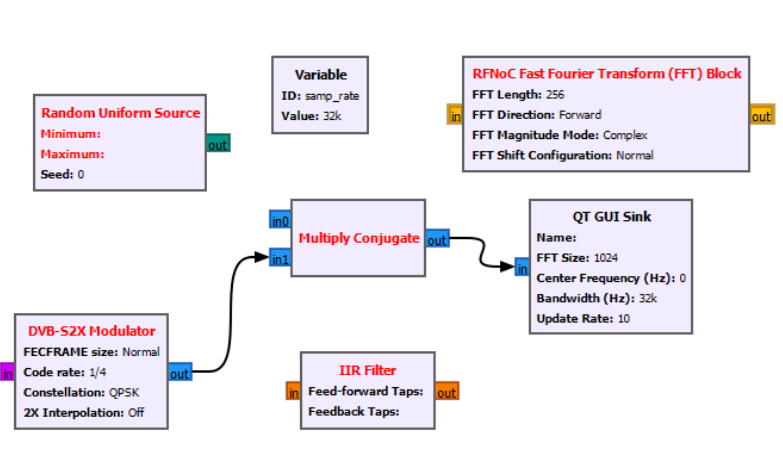
\includegraphics[width=\linewidth]{img/block-diagrams.png}
                 \caption{Blocks available}
                \label{fig:blocks_gnu}
            \end{figure}
        \end{column}
    \end{columns}
    % \begin{figure}
    %     \centering
    %     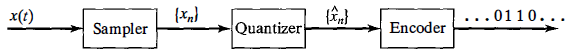
\includegraphics[width=0.7\linewidth]{img/PCM_steps.png}
    %     \caption{Block Diagram for a PCM System}
    %     \label{fig:enter-label}
    % \end{figure}
	
\end{frame}

%----------------------------------------------------------------------------------------
% \subsection{Sampling}\section{Resources}
\begin{frame}
	\frametitle{Resources}
    
\begin{columns}
        % First column
        \begin{column}{0.5\textwidth}
     \begin{itemize}
    \item Library with various processing blocks available in
    \begin{enumerate}
     \item Inside the GUI;
     \item C++;
     \item Python.
    \end{enumerate}
     \end{itemize}
     
        \end{column}
        
        % Second column
        \begin{column}{0.5\textwidth}
            \begin{figure}[t]
                \centering
                
\includegraphics[width=\linewidth]{img/GNU_radio_logo.png}
                 %\caption{Blocks Available}
                \label{fig:gnu_radio_logo}
            \end{figure}
            \begin{figure}
                \centering
                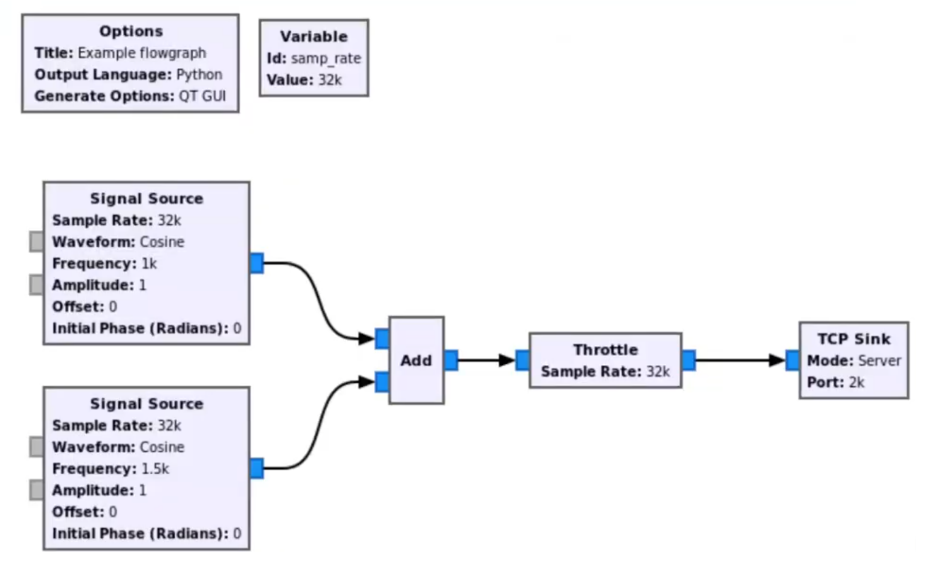
\includegraphics[width=\linewidth]{img/flowgraph example.png}
                 \caption{Flowgraph example}
                \label{fig:enter-label}
            \end{figure}
        \end{column}
    \end{columns}
    % \begin{figure}
    %     \centering
    %     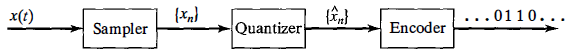
\includegraphics[width=0.7\linewidth]{img/PCM_steps.png}
    %     \caption{Block Diagram for a PCM System}
    %     \label{fig:enter-label}
    % \end{figure}
	
\end{frame}


%----------------------------------------------------------------------------------------

\begin{frame}
	\frametitle{Resources}
    
\begin{columns}
        % First column
        \begin{column}{0.5\textwidth}
     \begin{itemize}
    \item Library with various processing blocks available in
    \begin{enumerate}
     \item Inside the GUI;
     \item C++;
     \item Python.
    \end{enumerate}
     \end{itemize}
     
        \end{column}
        
        % Second column
        \begin{column}{0.5\textwidth}
            % \begin{figure}[t]
            %     \centering
            %     
\includegraphics[width=\linewidth]{img/GNU_radio_logo.png}
            %      %\caption{Blocks Available}
            %     \label{fig:gnu_radio_logo}
            % \end{figure}

 \begin{figure}
        \centering
        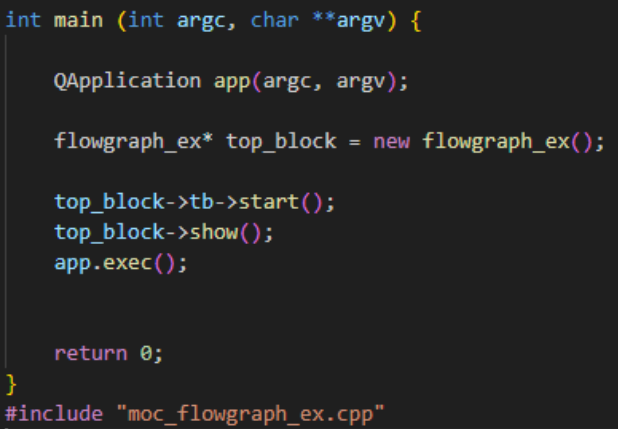
\includegraphics[width=0.5\linewidth]{img/c++.png}
        \caption{C++ output}
        \label{fig:enter-label}
    \end{figure}
                \begin{figure}
        \centering
        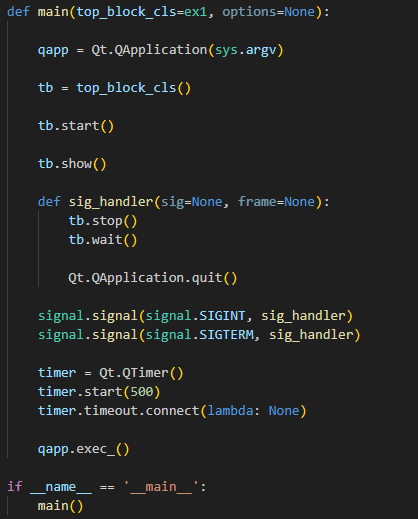
\includegraphics[width=0.3\linewidth]{img/python.png}
        \caption{Python output}
        \label{fig:enter-label}
    \end{figure}
            % \begin{figure}
            %     \centering
            %     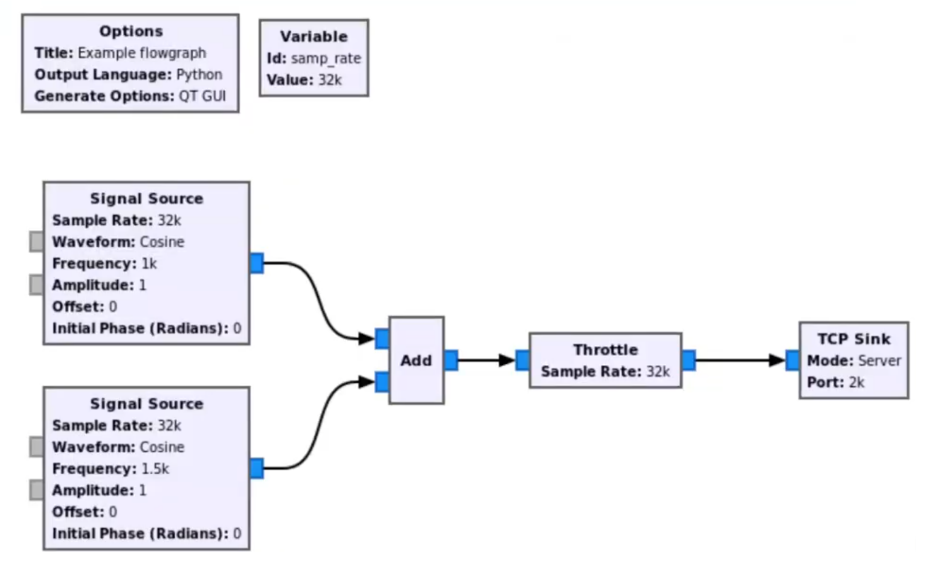
\includegraphics[width=\linewidth]{img/flowgraph example.png}
            %      \caption{Flowgraph example}
            %     \label{fig:enter-label}
            % \end{figure}
        \end{column}
    \end{columns}
    % \begin{figure}
    %     \centering
    %     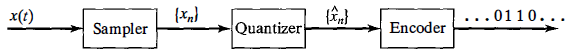
\includegraphics[width=0.7\linewidth]{img/PCM_steps.png}
    %     \caption{Block Diagram for a PCM System}
    %     \label{fig:enter-label}
    % \end{figure}
	
\end{frame}


%----------------------------------------------------------------------------------------

% \begin{frame}
% 	\frametitle{Resources}
    
% \begin{columns}
%         % First column
%         \begin{column}{0.5\textwidth}
   
%         \end{column}
        
%         % Second column
%         \begin{column}{0.5\textwidth}
         
%             % \begin{figure}
%             %     \centering
%             %     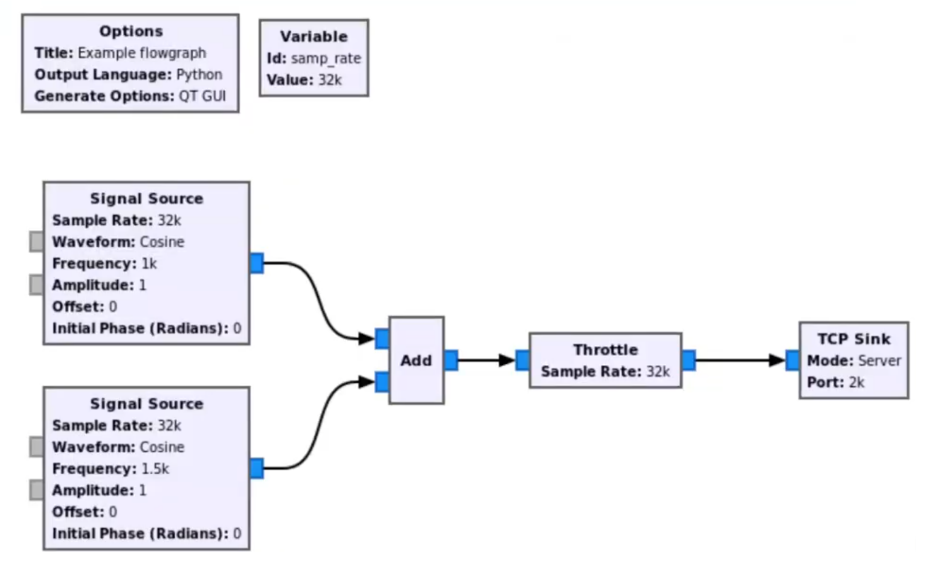
\includegraphics[width=\linewidth]{img/flowgraph example.png}
%             %      \caption{Flowgraph example}
%             %     \label{fig:enter-label}
%             % \end{figure}
%         \end{column}
%     \end{columns}
%     % \begin{figure}
%     %     \centering
%     %     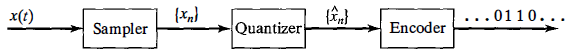
\includegraphics[width=0.7\linewidth]{img/PCM_steps.png}
%     %     \caption{Block Diagram for a PCM System}
%     %     \label{fig:enter-label}
%     % \end{figure}
	
% \end{frame}


%----------------------------------------------------------------------------------------



\section{Applications}
\begin{frame}
	\frametitle{Applications}
    
\begin{columns}
        % First column
        \begin{column}{0.5\textwidth}
     \begin{itemize}
    \item Defense and Security:
    \begin{enumerate}
    \item Signal intelligence and wireless security assessments;
    \item RF jamming detection and countermeasure development;
    \end{enumerate}
     \end{itemize}
     
        \end{column}
        
        % Second column
        \begin{column}{0.5\textwidth}
            \begin{figure}[]
                \centering
                
\includegraphics[width=\linewidth]{img/GNU_radio_logo.png}
                 %\caption{Blocks Available}
                \label{fig:gnu_radio_logo}
            \end{figure}
            \begin{figure}
                \centering
                
\includegraphics[width=0.5\linewidth]{img/applications/intelligence.png}
                %\caption{Defense}
                \label{fig:enter-label}
            \end{figure}
        \end{column}
    \end{columns}
\end{frame}

%----------------------------------------------------------------------------------------
%\subsection{Encoding}
%\section{Applications}
\begin{frame}
	\frametitle{Applications}
    
\begin{columns}
        % First column
        \begin{column}{0.5\textwidth}
     \begin{itemize}
    \item Telecommunications:
    \begin{enumerate}
     \item 5G and IoT prototyping and testing wireless communication protocols;
     \item Dynamic spectrum access and cognitive radio development.
    \end{enumerate}

     \end{itemize}
     
        \end{column}
        
        % Second column
        \begin{column}{0.5\textwidth}
            \begin{figure}[]
                \centering
                
\includegraphics[width=\linewidth]{img/GNU_radio_logo.png}
                 %\caption{Blocks Available}
                \label{fig:gnu_radio_logo}
            \end{figure}
            \begin{figure}
                \centering
                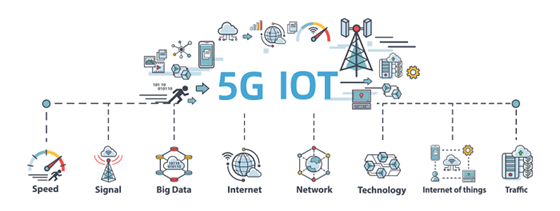
\includegraphics[width=\linewidth]{img/iot_5g.png}
                %\caption{Caption}
                \label{fig:enter-label}
            \end{figure}
        \end{column}
    \end{columns}
\end{frame}

%----------------------------------------------------------------------------------------

\begin{frame}
	\frametitle{Applications}
    
\begin{columns}
        % First column
        \begin{column}{0.5\textwidth}
     \begin{itemize}
    \item Satellite Communication:
    \begin{enumerate}
        \item Decoding telemetry and data from satellites including Cubesas and weather satellites.
        \item Supports ground station operations and satellite tracking.
    \end{enumerate}
     \end{itemize}
     
        \end{column}
        
        % Second column
        \begin{column}{0.5\textwidth}
            \begin{figure}[]
                \centering
                
\includegraphics[width=\linewidth]{img/GNU_radio_logo.png}
                 %\caption{Blocks Available}
                \label{fig:gnu_radio_logo}
            \end{figure}
            \begin{figure}
                \centering
                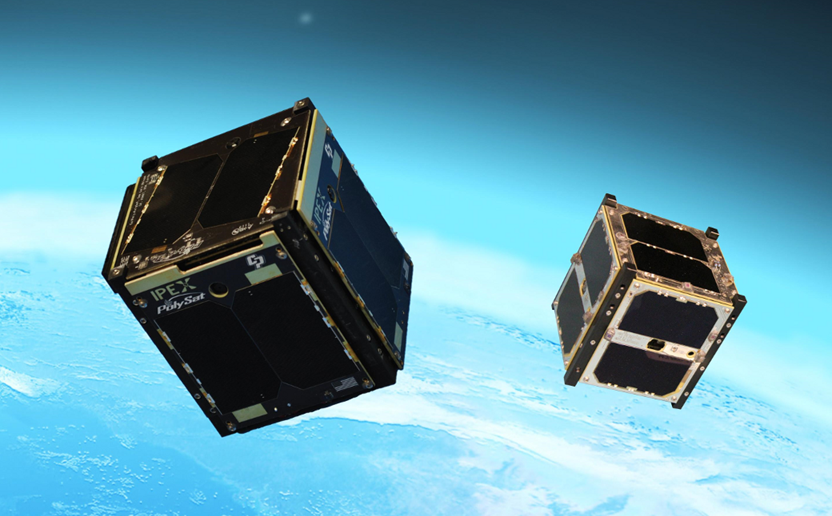
\includegraphics[width=\linewidth]{img/applications/satellite.png}
                %\caption{Caption}
                \label{fig:enter-label}
            \end{figure}
        \end{column}
    \end{columns}
\end{frame}

%----------------------------------------------------------------------------------------
%\section{Applications}
\begin{frame}
	\frametitle{Applications}
    
\begin{columns}
        % First column
        \begin{column}{0.5\textwidth}
     \begin{itemize}
    \item Academic and Research:
    \begin{enumerate}
        \item Lectures on Digital Signal Processing (DSP) and communication Systems.
        \item Valuable tool for prototyping new algorithms and conducting experiments on (RF) systems.
    \end{enumerate}
     \end{itemize}
     
        \end{column}
        
        % Second column
        \begin{column}{0.5\textwidth}
            \begin{figure}[]
                \centering
                
\includegraphics[width=\linewidth]{img/GNU_radio_logo.png}
                 %\caption{Blocks Available}
                \label{fig:gnu_radio_logo}
            \end{figure}
            \begin{figure}
                \centering
                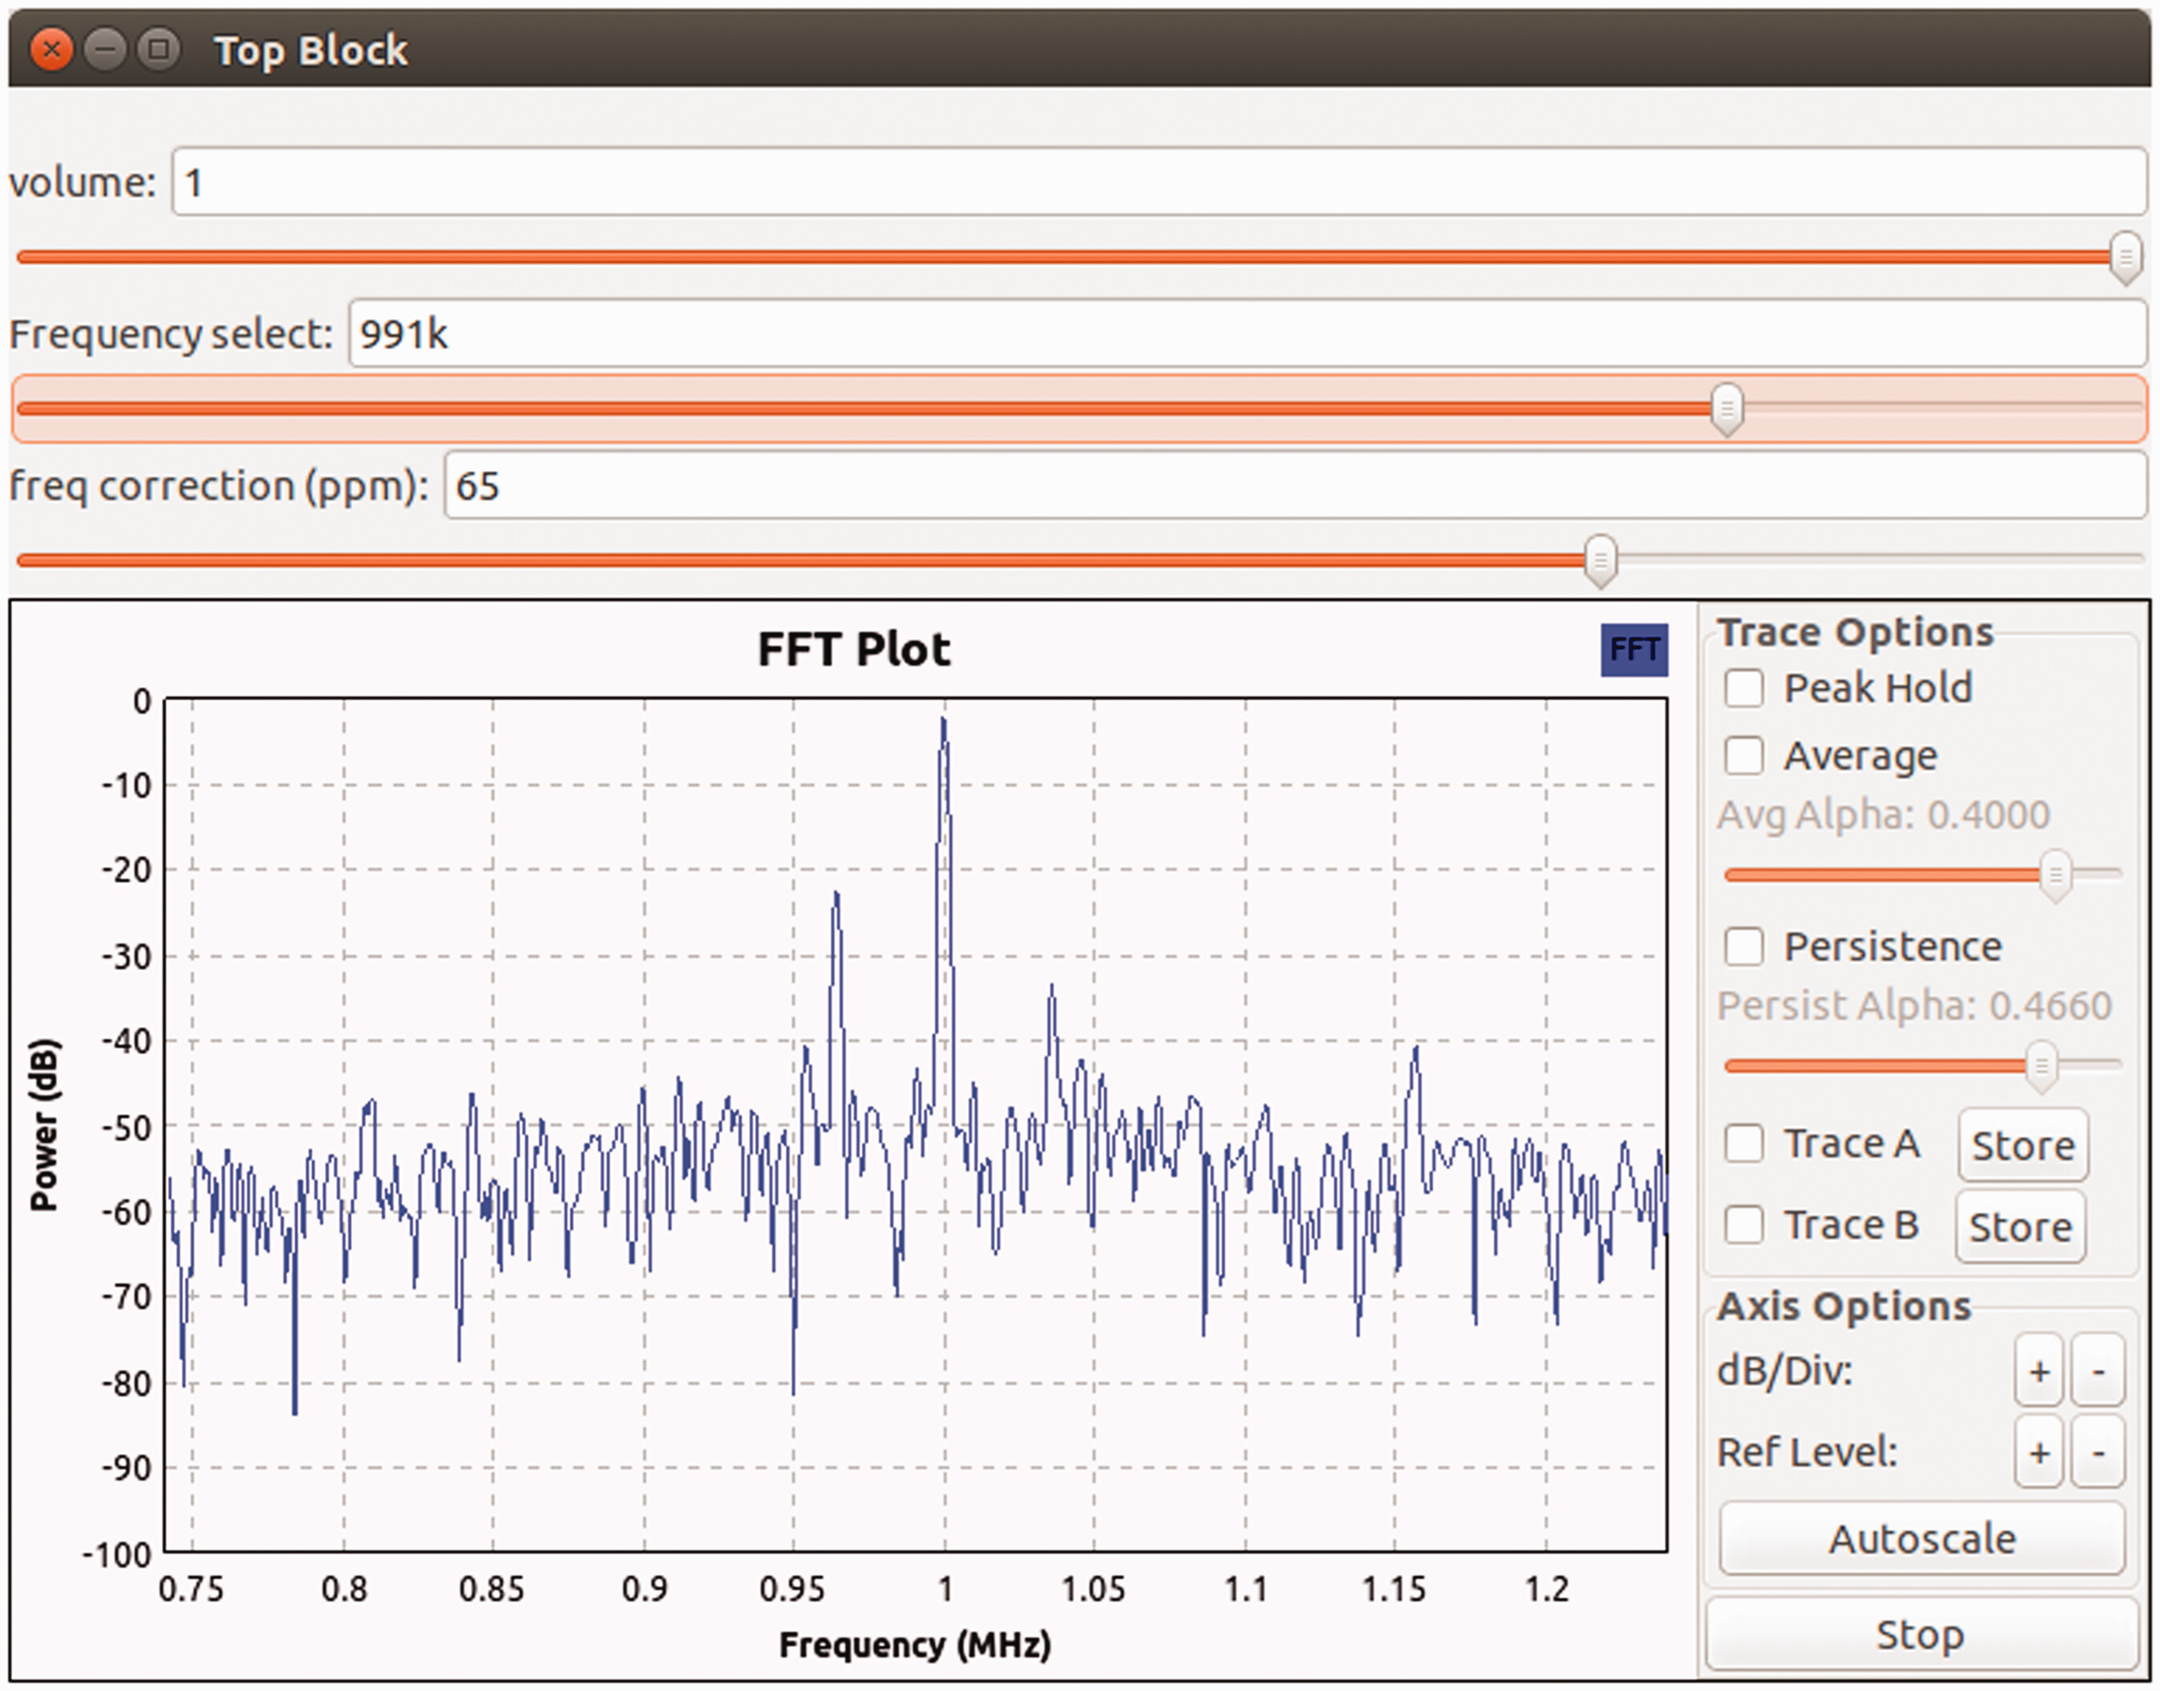
\includegraphics[width=.7\linewidth]{img/applications/learning.png}
                %\caption{Caption}
                \label{fig:enter-label}
            \end{figure}
        \end{column}
    \end{columns}
\end{frame}

%----------------------------------------------------------------------------------------
%\section{Applications}
\section{Practise}
\begin{frame}
	\frametitle{First Exercise}
    
\begin{figure}
    \centering
    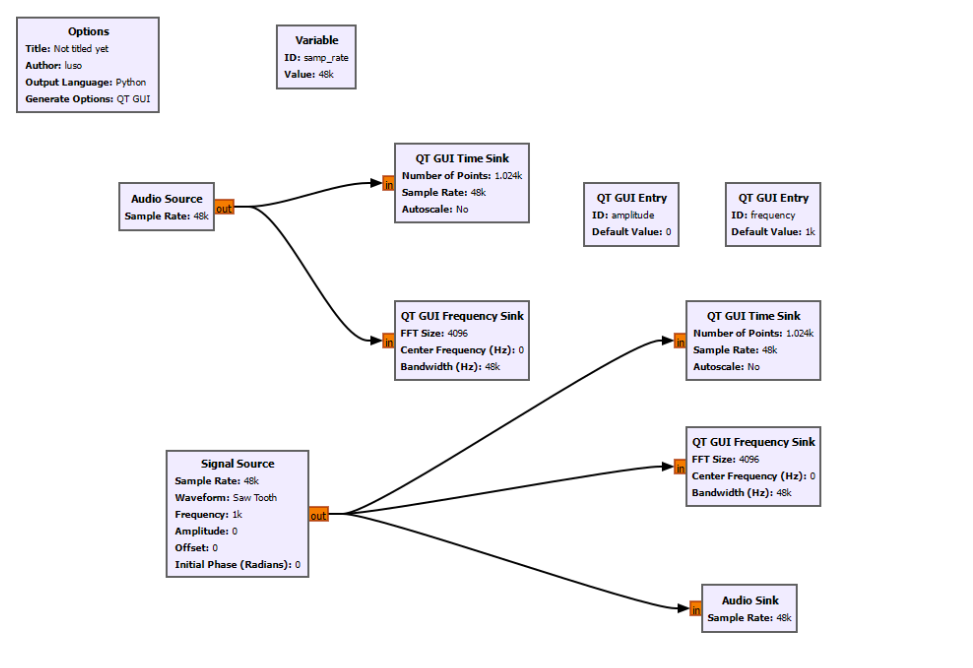
\includegraphics[width=0.8\linewidth]{img/applications/primeiro exercicio.png}
   % \caption{Caption}
    \label{fig:enter-label}
\end{figure}
\end{frame}

\section{Encoding} % Seções são adicionadas para organizar sua apresentação em blocos discretos, todas as seções e subseções são automaticamente exibidas no índice como uma visão geral da apresentação, mas NÃO são exibidas como slides separados.

%----------------------------------------------------------------------------------------

% \begin{frame}{Uniform PCM}
%     \begin{figure}
%         \centering
%         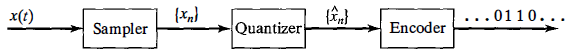
\includegraphics[width=0.7\linewidth]{img/PCM_steps.png}
%         %\caption{Block Diagram of a PCM System}
%         \label{fig:enter-label}
%     \end{figure}
%    \begin{align*}
%        \Delta = \frac{2x_{max}}{N} = \frac{x_{max}}{2^{\nu -1}}
%    \end{align*}
% \end{frame}

% %----------------------------------------------------------------------------------------
% \begin{frame}{$\mu$-law Compander}
%     \begin{figure}
%         \centering
%         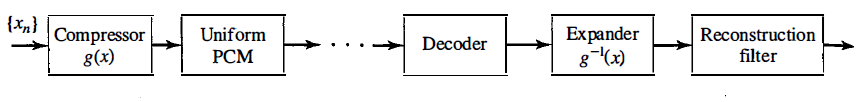
\includegraphics[width=0.7\linewidth]{img/non-unifor_PCM.png}
%         %\caption{Block Diagram of PCM}
%         \label{fig:block_pcm1}
%     \end{figure}
%     \begin{columns}

%          \column{0.48\textwidth}  % First column
%  \begin{figure}
%         \centering
%         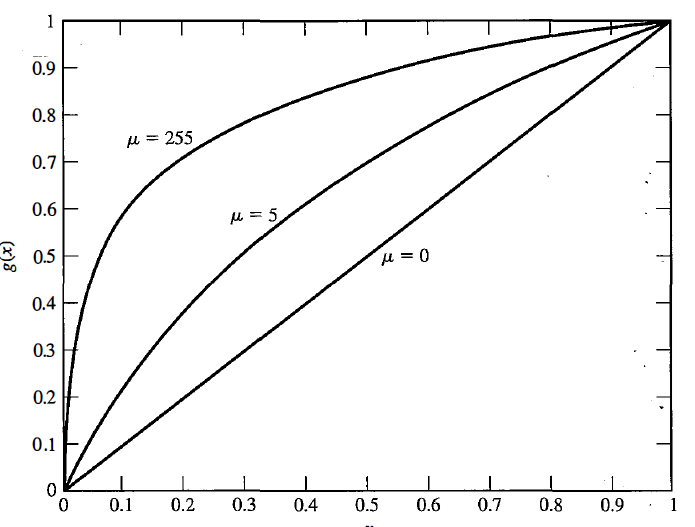
\includegraphics[width=1\linewidth]{img/mu-coding.png}
%         %\caption{Block Diagram of PCM}
%         \label{fig:u-law}
%     \end{figure}
%    \column{0.48\textwidth}  % First column
%     \begin{align*}
%        g(x) = \frac{\log (1+ \mu |x|)}{\log (1+\mu)} \text{sign}(x)
%    \end{align*}
%     \end{columns}
% \end{frame}

% %----------------------------------------------------------------------------------------
% \begin{frame}{A-law Compander}
%     \begin{figure}
%         \centering
%         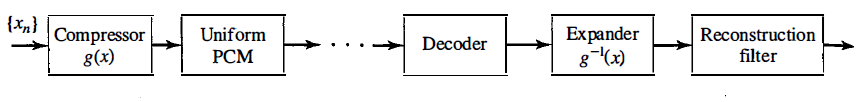
\includegraphics[width=0.7\linewidth]{img/non-unifor_PCM.png}
%         % \caption{Diagrama de blocos do PCM}
%         \label{fig:block_pcm}
%     \end{figure}
%        \begin{columns}

%          \column{0.48\textwidth}  % First column
%  \begin{figure}
%         \centering
%         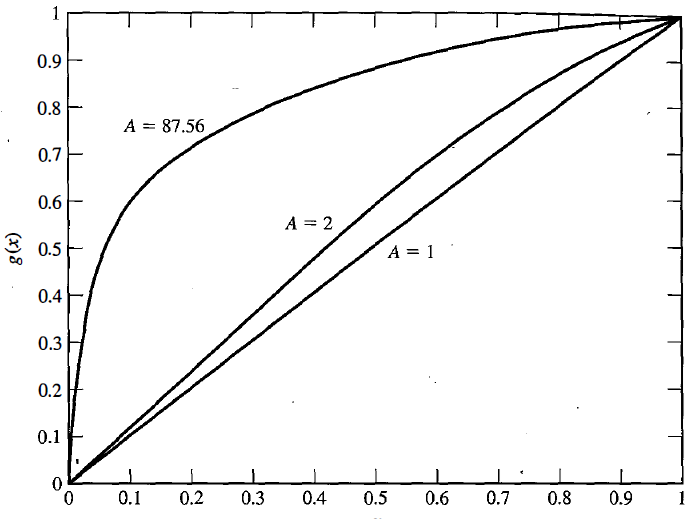
\includegraphics[width=1\linewidth]{img/A-coding.png}
%         % \caption{Diagrama de blocos do PCM}
%         \label{fig:a-law}
%     \end{figure}
%    \column{0.48\textwidth}  % First column
%     \begin{align*}
%        g(x) = \frac{1 +\log A |x|}{1 +\log A} \text{sign}(x)
%    \end{align*}
%     \end{columns}
% \end{frame}

%----------------------------------------------------------------------------------------
%\section{Exemplos com código} % Seções são adicionadas para organizar sua apresentação em blocos discretos, todas as seções e subseções são automaticamente exibidas no índice como uma visão geral da apresentação, mas NÃO são exibidas como slides separados.


%----------------------------------------------------------------------------------------
    \begin{frame}[fragile]
    \frametitle{Computing the Histrogram}
    \begin{columns}

         \column{0.48\textwidth}  % First column
    \begin{roundedcodebox}
    \begin{python}
#-----------------------------------
##   Compute a histogram of an image.
#   FAON - Jan 14th, 2023.
#-----------------------------------
def Compute_an_image_histogram(image, Bins):          
    N, M = image.shape  
    histogram = np.zeros((256), dtype = int)             
    histogram_Bins = np.zeros((Bins), dtype = int)
    if( Bins < 256):
        bins_step = 256.0 / Bins        
        for n in range(N):
          for m in range(M):
            histogram[image[n, m]]+= 1   
    \end{python}
\end{roundedcodebox}
   \column{0.48\textwidth}  % First column
    \begin{roundedcodebox}
    \begin{python}  
      if( Bins == 256 ): # In that case we have already computed histogram_Bins.
        histogram_Bins = histogram
    else:
        k = 0
        i=0
        while i < 256: 
            while ( (i >= (int) ( k * bins_step + 0.5) ) and (i < (int) (  (k + 1) * bins_step + 0.5 ) )):
                histogram_Bins[k] += histogram[i] 
                i += 1                 
            k +=1                 
    return histogram_Bins    
      \end{python}
\end{roundedcodebox}
    \end{columns}
\end{frame}

%----------------------------------------------------------------------------------------
    \begin{frame}[fragile]
    \frametitle{CDF/Inversa/Probability/Shannon}
    \begin{columns}

         \column{0.48\textwidth}  % First column
    \begin{roundedcodebox}
    \begin{python}
def Compute_cdf(pdf, Bins):
    cdf = np.zeros((Bins), dtype = float)
    cdf[0] = pdf[0]
    for k in range(1, Bins):   
        cdf[k] = cdf[k-1]+pdf[k]
    return cdf  
#----------------------------------
def Compute_inverse_cdf(cdf, probability):
    N = cdf.shape[0]          
    for k in range(N): 
        if(cdf[k] > probability):
            return k
            '''
            if(k > 0):
                return k
            else:
                return 0  
            ''' 
     \end{python}
\end{roundedcodebox}
  \column{0.48\textwidth}  % First column
    \begin{roundedcodebox}
    \begin{python}  
def Compute_probability(pmf, x1, x2, Bins): 
    probability = 0
    if( x2 == Bins):
        x2 = x2 - 1
    for k in range(x1, x2 + 1):
        probability += pmf[k]
    return probability   
#----------------------------------
def Compute_Shannon_entropy(pmf, Bins):
    epsilon = 2.2e-16
    bins_entropy = 0
    for i in range(Bins):
        bins_entropy -= pmf[i] * np.log2(pmf[i] + epsilon)
    return bins_entropy
\end{python}
\end{roundedcodebox}
    \end{columns}
\end{frame}

 


%----------------------------------------------------------------------------------------

    \begin{frame}[fragile]
    \frametitle{Robust Mean Absolute Deviation}
    \begin{columns}

         \column{0.48\textwidth}  % First column
    \begin{roundedcodebox}
    \begin{python}
def Compute_Robust_Mean_Absolute
_Deviation(image):
    N, M = image.shape
    image_p100 = np.percentile(image, 10.0)
    image_p900 = np.percentile(image, 90.0)
    #-----------------------------
    Robust_Mean_Absolute_Deviation = 0  
    percentile_range_10_90_pixels
    _values = np.zeros((N * M), dtype = float)
    k = 0
    for n in range(N):
        for m in range(M):
            if( (image[n,m] >= image_p100) and (image[n, m] <= image_p900) ):                    
     \end{python}
\end{roundedcodebox}
  \column{0.48\textwidth}  % First column
    \begin{roundedcodebox}
    \begin{python}  
                percentile_range_10_90_pixels
                _values[k] = image[n,m]
                k += 1
    if(k == 0):
        k = 1       
    percentile_range_10_90_pixels
    _mean = np.mean(percentile_range_10_90_pixels
    _values)   
    Robust_Mean_Absolute_Deviation = np.sum( abs(percentile_range_10_90_pixels
    _values - percentile_range_10_90_pixels
    _mean), axis = None ) / (float) (k)         
    return Robust_Mean_Absolute_Deviation


\end{python}
\end{roundedcodebox}
    \end{columns}
\end{frame}

%----------------------------------------------------------------------------------------

    \begin{frame}[fragile]
    \frametitle{Split/Statistical}
    \begin{columns}

         \column{0.48\textwidth}  % First column
    \begin{roundedcodebox}
    \begin{python}
def split_population(image, x1, x2):
    N, M = image.shape 
    x_pop = np.zeros((3, N * M), dtype = int)
    k1 = 0
    k2 = 0
    k3 = 0
    for n in range(N):
        for m in range(M):
            if(image[n, m] <= x1):
                x_pop[0, k1] = image[n,m]
                k1 += 1
            elif ( (image[n,m] > x1) and (image[n, m] <= x2) ): 
                x_pop[1, k2] = image[n,m]  
                k2 += 1
            else:
                x_pop[2, k3] = image[n,m]  
                k3 += 1            
    population_size = [k1, k2, k3]  
    return population_size, x_pop 
     \end{python}
\end{roundedcodebox}
  \column{0.48\textwidth}  % First column
    \begin{roundedcodebox}
    \begin{python}  
def calculates_statistical_quantities
_of_a_population(x, x1, x2, N): 
    if( x1 == 0):
        M = x2 - x1 + 1
    else:
       M = x2 - x1          
    histogram = np.zeros((M), dtype = int)  
    #------------------------
    #   Compute the histogram using 256 bins.
    #------------------------
    if( x1 == 0):
        for n in range(N):
            histogram[x[n]] += 1  
    else:
        for n in range(N):
            histogram[x[n] - x1 - 1] += 1 
pmf = histogram/N
\end{python}
\end{roundedcodebox}
    \end{columns}
\end{frame}

%----------------------------------------------------------------------------------------

\begin{frame}[fragile]
    \frametitle{Features}
\begin{columns}
  \column{0.48\textwidth}  % First column
    \begin{roundedcodebox}
    \begin{python}  
    #---------------------------
    # Statistical mean.
    #---------------------------
    sum = 0.0
    for k in range(M):    
         sum +=  (k + x1) * pmf[k]
    mean = sum
    #---------------------------
    # Statistical variance.
    #---------------------------
    sum = 0.0
    for k in range(M):    
         sum +=  ((k + x1 - mean)**2.0) * pmf[k]
    variance = sum    
\end{python}
\end{roundedcodebox}
  \column{0.48\textwidth}  % First column
    \begin{roundedcodebox}
    \begin{python}  
    #---------------------------
    # Statistical skewness.
    #---------------------------
    sum = 0.0
    for k in range(M):    
         sum +=  ((k + x1 - mean)**3.0) * pmf[k]
    central_moment_3 = sum 
    skewness = central_moment_3 /variance**1.5       
    #---------------------------
    # Statistical Kurtosis.
    #---------------------------
    sum = 0.0
    for k in range(M):    
         sum +=  ((k + x1 - mean)**4.0) * pmf[k]
    central_moment_4 = sum 
    kurtosis = central_moment_4 /variance**2.0              
    return mean, variance, skewness, kurtosis   

\end{python}
\end{roundedcodebox}
    \end{columns}
\end{frame}

%----------------------------------------------------------------------------------------

\begin{frame}[fragile]
    \frametitle{Statistical Features - Code Output}
\begin{columns}
  \column{0.48\textwidth}  % First column
    \begin{roundedcodebox}
    \begin{python}  
    def Compute_Statistical_Features(image, Bins):        
    features = []     
    N, M = image.shape  
    image_number_of_pixels = float(N * M) 
    #----------------------------
    # Compute image's hitogram using the developed method.
    #----------------------------
    histogram = Compute_an_image_histogram(image, Bins)        
    #histogram_in_ascending_order = np.sort(histogram)               
    #----------------------------
    # Build the Power Mass Function.
    #----------------------------
    pmf = histogram / image_number_of_pixels
    cdf = Compute_cdf( pmf, Bins)        
\end{python}
\end{roundedcodebox}
  \column{0.48\textwidth}  % First column
    \begin{roundedcodebox}
    \begin{python}  
    #---------------------------
    # It computes statistical features of Type I.
    #---------------------------
    image_min = np.min(image) 
    image_max = np.max(image)
    image_mean = round(np.mean(image), 3) 
    image_median = (int) (np.median(image))
    image_std = round(np.std(image), 3)  
    image_var = round(np.var(image), 3) 
    #---------------------------   
    image_mode = np.argmax(pmf)
    image_skew = round(scipy.stats.skew(image, axis = None), 3)
    image_kurtpsis = round(scipy.stats.kurtosis(image, axis = None),3)
    square_range = round((image_max - image_min)**2, 3)
\end{python}
\end{roundedcodebox}
    \end{columns}
\end{frame}

%----------------------------------------------------------------------------------------

\begin{frame}[fragile]
    \frametitle{Features of Type II}
\begin{columns}
  \column{0.48\textwidth}  % First column
    \begin{roundedcodebox}
    \begin{python}  
    #---------------------------   
    # Compute Shannon entropy 2
    #---------------------------   
    Shannon_entropy = round(Compute_Shannon_entropy(pmf, Bins), 3)
    #---------------------------         
    # Normalized energy.
    #---------------------------   
    image_norm_energy = round((np.sum( image**2, axis = None ) / image_number_of_pixels),3)
    #---------------------------   
    # Root-Mean-Square (RMS) value.
    #---------------------------   
    image_rms = round(np.sqrt(image_norm_energy),3)  
\end{python}
\end{roundedcodebox}
  \column{0.48\textwidth}  % First column
    \begin{roundedcodebox}
    \begin{python}  
    #---------------------------   
    # Compute the statistics Features of Type II.
    #---------------------------   
           
    #---------------------------   
    # Compute the percentiles from image using Numpy.
    #---------------------------   
    image_p75 = np.percentile(image, 7.5)
    image_p150 = np.percentile(image, 15.0)      
    image_p850 = np.percentile(image, 85.0)        
    image_p925 = np.percentile(image, 92.5)  
\end{python}
\end{roundedcodebox}
    \end{columns}
\end{frame}

%----------------------------------------------------------------------------------------
\begin{frame}[fragile]
    \frametitle{Features of Type III}
\begin{columns}
  \column{0.48\textwidth}  % First column
    \begin{roundedcodebox}
    \begin{python}  
    # It computes statistical features of Type III.
    #---------------------------  
      
    #---------------------------
    # Compute image interquartile range.
    #---------------------------
    image_p250 = np.percentile(image, 25.0)
    image_p750 = np.percentile(image, 75.0)      
    image_interquartile_range = image_p750 - image_p250
    #---------------------------
    # Mean Absolute Deviation from the mean.
    #---------------------------
    image_abs_deviation_from_the_mean = round((np.sum( np.abs(image - image_mean), axis = None ) / image_number_of_pixels),3)
    #---------------------------
    
\end{python}
\end{roundedcodebox}
  \column{0.48\textwidth}  % First column
    \begin{roundedcodebox}
    \begin{python}  
    # Mean Absolute Deviation from the median.
    #---------------------------
    image_deviation_from_the_median = round((np.sum((image - image_median), axis = None ) / image_number_of_pixels),3)  
    #---------------------------
    # Compute image normalized uniformity from its histogram.
    #---------------------------        
    image_uniformity = round((np.sum( histogram**2, axis = None ) / image_number_of_pixels),3)          
    #---------------------------
    # Compute the Robust Mean Absolute Deviation (rMAD).
    #--------------------------- 
    Robust_Mean_Absolute_Deviation = round(Compute_Robust_Mean_Absolute
    _Deviation(image), 3)
    #---------------------------
   
\end{python}
\end{roundedcodebox}
    \end{columns}
\end{frame}

%----------------------------------------------------------------------------------------
\begin{frame}[fragile]
    \frametitle{Features of Type IV}
\begin{columns}
  \column{0.48\textwidth}  % First column
    \begin{roundedcodebox}
    \begin{python}  
    x1 = Compute_inverse_cdf(cdf, 0.333)
    x2 = Compute_inverse_cdf(cdf, 0.666)
    #---------------------------                
    # Splites the population. 
    #---------------------------      
    population_size, x_pop = split_population(image, x1, x2)
    population_threshold = (int) (image_number_of_pixels/3)
    threshold_deviation_1 = population_size[0] - population_threshold
    threshold_deviation_2 = population_size[1] - population_threshold  
    #threshold_deviation_3 = population_size[2] - population_threshold
    #---------------------------
    # Mean, variance, skeness and kurtosis of population 1.
    #---------------------------
\end{python}
\end{roundedcodebox}
  \column{0.48\textwidth}  % First column
    \begin{roundedcodebox}
    \begin{python}  
    x = x_pop[0,:]
    m1, v1, s1, k1 = calculates_statistical_quantities
    _of_a_population(x, 0, x1, population_size[0])
    m1 = round(m1, 3) 
    v1 = round(v1, 3) 
    s1 = round(s1, 3)     
    k1 = round(k1, 3)   
    #---------------------------
    # It computes mean, variance, skeness and kurtosis of population 2.
    x = x_pop[1,:]
    m2, v2, s2, k2 = calculates_statistical_quantities
    _of_a_population(x, x1, x2, population_size[1]) 
    m2 = round(m2, 3) 
    v2 = round(v2, 3) 
    s2 = round(s2, 3)     
    k2 = round(k2, 3)      
         
\end{python}
\end{roundedcodebox}
    \end{columns}
\end{frame}

%----------------------------------------------------------------------------------------
\begin{frame}[fragile]
    \frametitle{Features of Type IV}
\begin{columns}
  \column{0.48\textwidth}  % First column
    \begin{roundedcodebox}
    \begin{python}  
    #---------------------------
    # It computes mean, variance, skeness and kurtosis of population 2.
    #---------------------------
    x = x_pop[2,:]  
    m3, v3, s3, k3 = calculates_statistical_quantities
    _of_a_population(x, x2, Bins - 1, population_size[2])  
    m3 = round(m3, 3) 
    v3 = round(v3, 3) 
    s3 = round(s3, 3)     
    k3 = round(k3, 3) 
\end{python}
\end{roundedcodebox}
  \column{0.48\textwidth}  % First column
    \begin{roundedcodebox}
    \begin{python}  

\end{python}
\end{roundedcodebox}
    \end{columns}
\end{frame}

%----------------------------------------------------------------------------------------
\begin{frame}[fragile]
    \frametitle{Python}
\begin{columns}
  \column{0.48\textwidth}  % First column
    \begin{roundedcodebox}
    \begin{python}  
    
\end{python}
\end{roundedcodebox}
  \column{0.48\textwidth}  % First column
    \begin{roundedcodebox}
    \begin{python}  

\end{python}
\end{roundedcodebox}
    \end{columns}
\end{frame}

%----------------------------------------------------------------------------------------

% \begin{frame}[fragile]
%     \frametitle{C}
    
%     \begin{clang}
% #include <stdio.h>

% int main() {
%     int numero = 5;
%     int dobro = 2 * numero;
    
%     printf("O dobro de %d eh %d\n", numero, dobro);
%     return 0;
% }
%     \end{clang}
% \end{frame}

% %----------------------------------------------------------------------------------------
% \begin{frame}[fragile]
%     \frametitle{C++}
    
%     \begin{cpp}
% #include <iostream>
% using namespace std;

% int main() {
%     int numero = 5;
%     int dobro = 2 * numero;
    
%     cout << "O dobro de " << numero;
%     cout << " eh " << dobro << endl;
%     return 0;
% }
%     \end{cpp}
% \end{frame}

% %----------------------------------------------------------------------------------------
% \begin{frame}[fragile]
%     \frametitle{R}
    
%     \begin{rlang}
% # Função para calcular o dobro
% calcular_dobro <- function(x) {
%   return(2 * x)
% }

% # Testando a função
% numero <- 5
% resultado <- calcular_dobro(numero)
% print(paste("O dobro de", numero, "é", resultado))
%     \end{rlang}
% \end{frame}

% %----------------------------------------------------------------------------------------

% \begin{frame}[fragile]
%     \frametitle{Java}
    
%     \begin{java}
% public class Exemplo {
%     public static void main(String[] args) {
%         int numero = 5;
%         int dobro = 2 * numero;
        
%         System.out.println("O dobro de " + numero +
%                          " eh " + dobro);
%     }
% }
%     \end{java}
% \end{frame}
 % \section{Reconstruction} % Seções são adicionadas para organizar sua apresentação em blocos discretos, todas as seções e subseções são automaticamente exibidas no índice como uma visão geral da apresentação, mas NÃO são exibidas como slides separados.
\begin{frame}{Signal Reconstruction}
    \begin{figure}
        \centering
        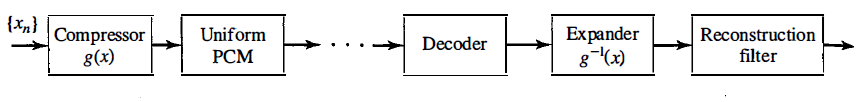
\includegraphics[width=0.7\linewidth]{img/non-unifor_PCM.png}
        % \caption{Diagrama de blocos do PCM}
        \label{fig:block_pcm}
    \end{figure}
       \begin{columns}

         \column{0.48\textwidth}  % First column
         Reconstruction Diagram
 \begin{figure}
        \centering
        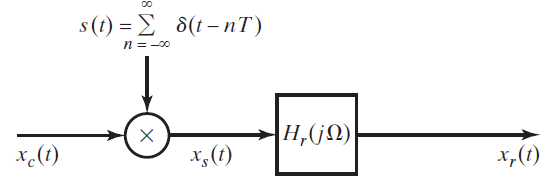
\includegraphics[width=1\linewidth]{img/reconstruction_3.png}
        % \caption{Diagrama de blocos do PCM}
        \label{fig:a-law}
    \end{figure}
    \column{0.48\textwidth}  % First column
Frequency Response and Reconstructed Signal
\begin{figure}
        \centering
        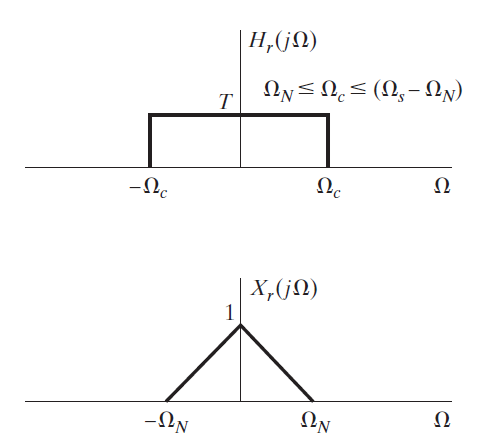
\includegraphics[width=.7\linewidth]{img/reconstruction_2.png}
        % \caption{Diagrama de blocos do PCM}
        \label{fig:a-law}
    \end{figure}
 
    \end{columns}
\end{frame}

%--------------------------------------------------------------------------------------------
\begin{frame}{Signal Reconstruction}
    \begin{figure}
        \centering
        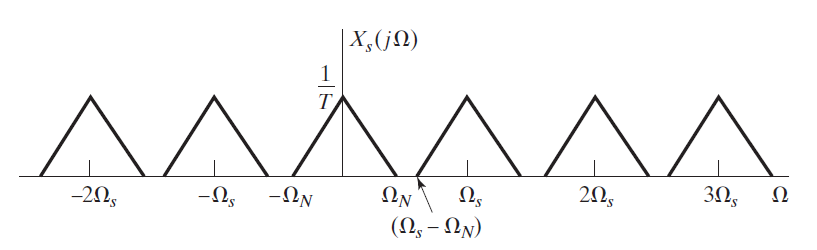
\includegraphics[width=0.7\linewidth]{img/reconstruction.png}
        % \caption{Diagrama de blocos do PCM}
        \label{fig:block_pcm}
    \end{figure}
\begin{figure}
        \centering
        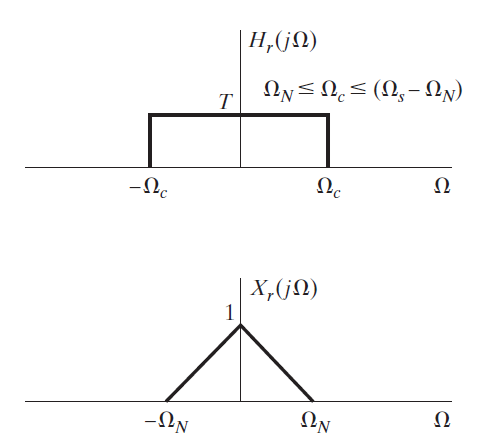
\includegraphics[width=.3\linewidth]{img/reconstruction_2.png}
        % \caption{Diagrama de blocos do PCM}
        \label{fig:a-law}
    \end{figure}
\end{frame}

% \begin{frame}{Referências}
%     \nocite{*}
%     \printbibliography[heading=none]
% \end{frame}

% Slide final
\begin{frame}
    \begin{center}
        {\Huge Demonstration}
    \end{center}
\end{frame}

\end{document}


